\begin{figure}[h!]
	\centering
	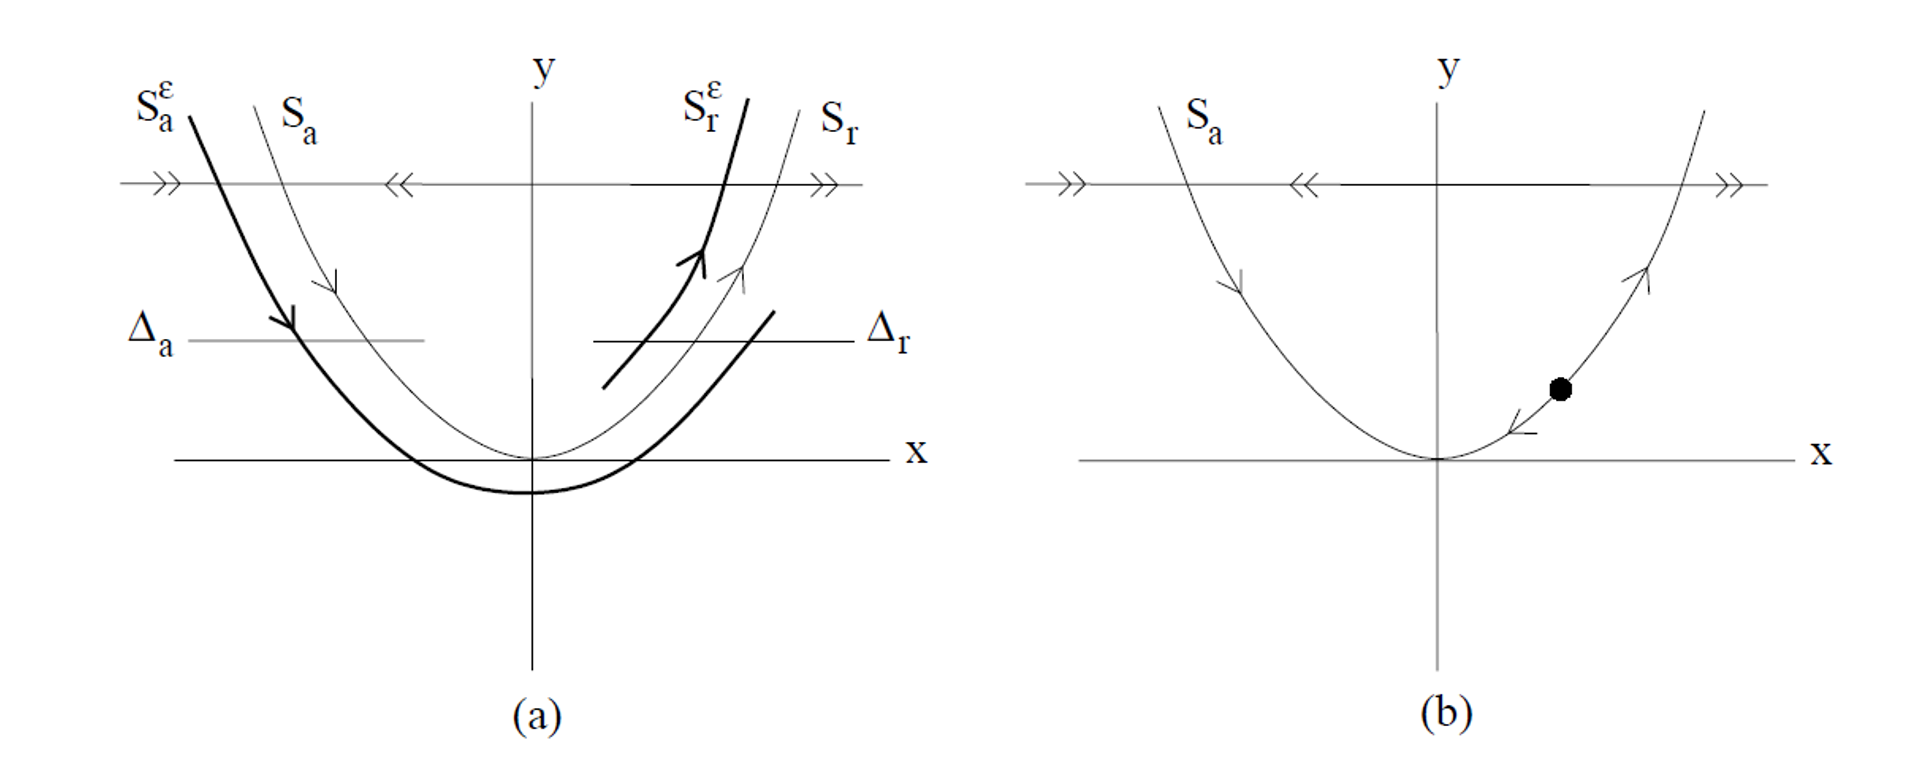
\includegraphics[height=5cm,width=8cm]{Canard_Point.png}
	\caption{The reduced flow where a) $\lambda=0$ and b) $\lambda>0$.}
	\label{fig: Canard Point}
\end{figure}\newpage



Considering the Van der Pol System as before:
\begin{equation}
\begin{aligned}
&x'=-y+x^2-\dfrac{x^3}{3},\\
&y'=\epsilon(x-1),\\
\end{aligned}
\tag{\ref{eq: Fast System}}
\end{equation}
we notice that the equilibrium of the system depends on the two nullclines $ x'=0$ and $y'=0$. These are in the shape of a cubic funcion and in the shape of a vertical line at $x=1$. 
The idea in this section is to replace the nullcline $x=1$ by $x = \lambda$. This can be seen as shifting the equilibrium of the system along the critical manifold $S$ by varying the parameter $\lambda$.
This gives rise to a generalised Van der Pol system:
\begin{equation}
\begin{aligned}
&x'=-y+x^2-\dfrac{x^3}{3},\\
&y'=\epsilon(x-\lambda).\\
\end{aligned}
\label{eq: canard system}
\end{equation}
In this section, the dynamics in system \ref{eq: canard system} is analysed. In order to do so, we need the definition of a canard.
\begin{definition}{\textbf{ Canard}}[\citealp{Kuehn}]
A trajectory of a fast-slow system is called a canard if it stays within $O(\epsilon)$ close to the repelling branch $S^r$ of the slow manifold $S$, for some time of $O(1)$ on the slow time scale $\tau = \epsilon t$.
\end{definition}
Furthermore, the following definition turns out to be useful as well:
\begin{definition}{\textbf{Maximal Canard}}[\citealp{Kuehn}] \label{maxcanard}
The trajectory passing through the intersection of $S^a$ and $S^r$ is called a maximal canard. 
\end{definition}
\begin{definition}{\textbf{Singular Canard}}
\end{definition}
The intuition of the canard problem close to a fold point is given in Figure \ref{fig: Canard Point}.
Equivalently to the analysis of the fold point in Section \ref{sec:the-van-der-pol-equation}, some nondegeneracy conditions are defined. These are, as before, applied at the fold point $(0,0)$. Note that in contrast to the nondegeneracy conditions in (\ref{NonDeg}), the transversality condition $g(0,0,0) \neq 0$ is not satisfied. Therefore higher order conditions on $g$ have to be employed, in particular these are nonzero derivatives of $g$ with respect to $x$ and $\lambda$. The fact that $g_x(0,0,0) \neq 0$ guarantees the existence of transversal intersection of the two nullclines, which is crucial in order to conclude persistence of the dynamics later on \citep{kuehn}. 
The nondegeneracy and transversality conditions for the canard case are  \citep{krupa2001},
\begin{equation}
f(0,0,0,0)=0, \ \pd{}{x}f(0,0,0,0)=0, \ g(0,0,0,0)=0, \label{eq: canard sing condition}
\end{equation}
\begin{equation}
\begin{aligned}
&\pd{^2}{x^2}f(0,0,0,0)\neq 0, \ \pd{}{y}f(0,0,0,0)\neq 0,\\
&\pd{}{x}g(0,0,0,0)\neq 0, \ \pd{}{\lambda}g(0,0,0,0)\neq 0. \label{eq: canard non-d condition}
\end{aligned}
\end{equation}
Now that these conditions have been defined we can consider, equivalent to the argument in Section \ref{sec: extended sys blowup}, the extended \vdp system,
\begin{equation}
\begin{aligned}
&x'=-y+x^2-\dfrac{x^3}{3},\\
&y'=\epsilon(x-\lambda),\\
&\epsilon'=0,\\
&\lambda'=0,\\
\end{aligned}
\label{eq: canard system}
\end{equation}
where the change in $\epsilon$ and $\lambda$ are constant. 
Now, for the remainder of the section, we apply the method of \citet{krupa2001} to the Van der Pol System. The canonical form for the Canard System is:
\begin{equation} \label{canardysy2var}
	\begin{aligned}
		x'&=-yh_1(x,y,\epsilon,\lambda)+x^2h_2(x,y,\epsilon,\lambda) + \epsilon h_3(x,y,\lambda,\epsilon)\\
                        &= -y + x^2 \left( 1- \frac{x}{3} \right),\\
		y'&=\epsilon(xh_4(x,y,\epsilon,\lambda)-\lambda h_5(x,y,\epsilon,\lambda) + y h_6(x,y,\lambda,\epsilon)) \\
                        &= \epsilon( x- \lambda).
	\end{aligned}
\end{equation}
It follows that $h_1 = 1$, $h_2 = 1-\frac{x}{3}$, $h_3=0$, $h_4 =1$, $h_5=1$ and $h_6=0$.
It is possible to find a $\lambda>0$, for which an equilibrium on the repelling branch $S_r$ exists for the reduced dynamics.
The following definition can be made in order to simplify the following computations:

\begin{align*}
a_1=\pd{}{x}h_3(0,0,0,0)=& 0 \ \ \
a_2=\pd{}{x}h_1(0,0,0,0)= 0\ \ \ 
a_3=\pd{}{x}h_2(0,0,0,0)=-\frac{1}{3}\\
a_4&=\pd{}{x}h_4(0,0,0,0)=0\ \ \
a_5=h_6(0,0,0,0)=0.
\end{align*}
Furthermore, we can define the quantity:
\begin{align*}
A=-a_2+3a_3-(2a_4+2a_5)=-1,
\end{align*}
which is important in the following analysis, in particular for $A \neq 0$ \citep{krupa2001}. 
Similar to the procedure in Section \ref{sec: VDP Blowup}, sections of the dynamical system can be defined, in order to monitor the in- and outgoing trajectories. In this case we are interested in two sections of the neighbourhood $U$, defined as in Section \ref{sec: VDP Blowup}, that monitor $S^a$ and $S^r$ close to the fold point.
Let $ \Delta_a = \{ (x,\rho^2), x \in  I_a \}$ and $\Delta_r= \{ (x,\rho^2), x \in  I_r \}$, where $I_a,I_r$ are intervals on the real line and $\rho$ is sufficiently small.
Futhermore, define $q_a$ to be the point on $\Delta_a$ that belongs to the attracting branch $S^a$, while $q_r$ is equivalently defined as the point on $\Delta_r$ that corresponds to $S^r$. Finally, we are in the position to define the transition map $\pi: \Delta^a \to \Delta^r$, compare to Section \ref{sec: VDP Blowup}.
Following this, \citet{krupa2001} discuss the existence of a critical value for $\lambda$ (denoted $\lambda_c$), where the two branches $S_r$ and $S_a$ must connect in a smooth fashion.  
The transition map $\pi$ has to map the point $q_a$ to $q_r$, if the branches are connected, and the trajectory passing through the fold point is called the maximal canard, see Definition \ref{maxcanard}
The following theorem describes the technical details involved, and some of the results are derived by the following analysis.
\begin{theorem}[\cite{krupa2001}]
	Assume that system (3.1) satisfies the defining non-degeneracy conditions (Equations \ref{eq: canard sing condition} and \ref{eq: canard non-d condition}) of a canard point. Assume that the solution $ x_0(t) $ of the reduced problem connects $ S_a $ to $ S_r $. Then there exists $ \epsilon_0 > 0 $ and a smooth function $\lambda_c(\sqrt{\epsilon})$ defined on $ [0, \epsilon_0] $ such that for $\epsilon \in (0, \epsilon_0)$ the following assertions hold:
	\begin{itemize}
		\item $ \pi(q_{a,\epsilon})=q_{r,\epsilon} $ iff $ \lambda=\lambda_c(\sqrt{\epsilon}) $.\\
		\item The function $ \lambda_c $ has the expansion
		 \begin{equation*}
			\lambda_c(\sqrt{\epsilon})=-\epsilon(\frac{a_1+a_5}{2}+\frac{A}{8})+O(\epsilon^\frac{3}{2}).
			\end{equation*}
			\item The transition map $\pi$ is defined only for $\lambda$ in an interval around $ \lambda_c(\sqrt{\epsilon}) $ of width $ O(\exp(-\frac{c}{\epsilon})) $ fo some $ c>0 $.
			$$ \pd{}{\lambda}(\pi(q_{a,\epsilon})-q_{r,\epsilon})|_{\lambda=\lambda_c(\sqrt{\epsilon})}>0  $$
		
	\end{itemize}
\label{Theorem 3.1}
\end{theorem}
%Consider Canard cycles and center manifolds / Freddy Dumortier, Robert Roussarie. for more details on canards in \vdp. ++++++Kieran, what do you mean here+++++
%



\subsection{Canard Blow-up}
Now similarly to Section \ref{sec: VDP Blowup}, we consider a transformations of the coordinate system in order to analyse the dynamics in the neighbourhood of the non-hyperbolic equilibrium induced by the canard point. %(++++++ is the eq. induced by lambda??++++).
 The transformations are taken from \citep{krupa2001} and are,
\begin{equation}
x=\bar{r}\bar{x}, \ y=\bar{r}^2y, \ \epsilon=\bar{r}^2\bar{\epsilon}, \ \lambda=\bar{r}\bar{\lambda}.
\end{equation}
Now that we have established these transformation, the charts $K_1$ and $K_2$ can be introduced,  but it is not necessary to consider the third chart, $K_3$. Since the attracting slow manifold connects to the repelling slow manifold, the flow will `bend back' from $K_2$ into $K_1$ instead of leaving the neighbourhood $U$ in the direction of the fast flow, which was described by $K_3$ in Section \ref{sec: VDP Blowup}. 
This pheonomenon can be observed in Figure \ref{fig: flow in canard}, where the trajectory stays close to $S^r$ after passing the fold point.
\begin{figure}[h!]
	\centering
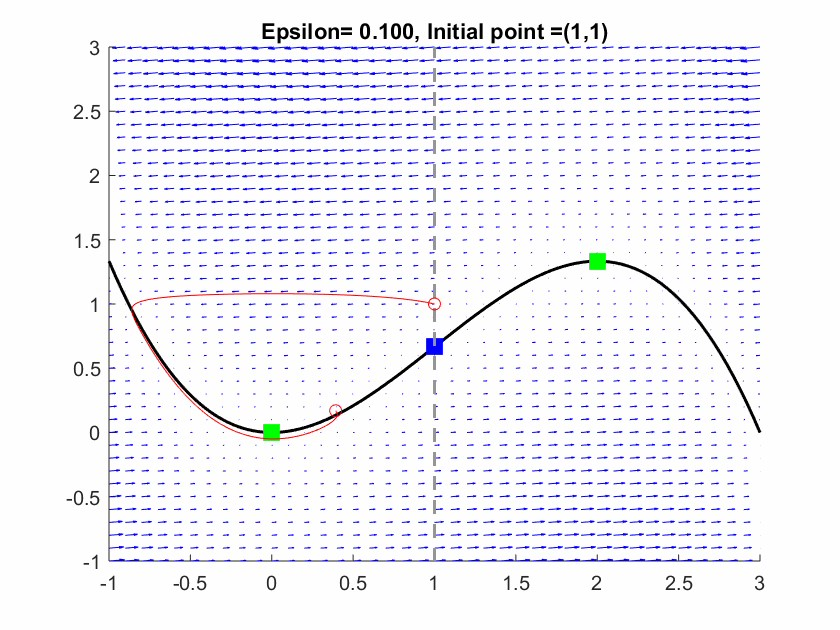
\includegraphics[width=8cm, height=6cm]{Images/vdPhopf-Moment-bendback}
	\caption{The \vdp system for the canard case.}
	\label{fig: flow in canard}
\end{figure}\newpage
Again, equivalently to the procedure in Section \ref{sec: VDP Blowup}, we can define the coordinate transformation for the charts. Note, that in contrast to the generic Blow-Up in Section \ref{sec: VDP Blowup}, the coordinate system is now in $\mathbf{R}^4$, and not in $\mathbf{R}^3$. In chart $K_1$, $y_1=1$, while in $K_2$, $\epsilon_1=1$ and then:
\begin{subequations}
	\begin{align}
	&x=r_1x_1, \ y=r_1^2, \ \epsilon=r_1^2\epsilon_1, \ \lambda=r_1\lambda_1 \label{eq: coordiante K1}\\ 
	&x=r_2x_2, \ y=r_2^2y_2, \ \epsilon=r^2_2, \ \lambda=r_2\lambda_2 \label{eq: coordinate K2}.
	\end{align}
\end{subequations}
Furthermore, we can define the coordinate change between the two charts as follows:
\begin{lemma}
Let $\kappa_{12}$ denote the change of coordinates from $K_1$ to $K_2$. Then $\kappa_{12}$ is given by
\begin{align*}
x_2 = x_1 \epsilon_1^{-1/2}, \ \ \ y_2 = \epsilon_1^{-1}, \ \ \ r_2 = r_1 \epsilon_1^{1/2}, \ \ \ \lambda_2 = \epsilon_1^{-1/2} \lambda_1,
\end{align*}
for $\epsilon_1 >0$.
Similarly $\kappa_{21}=\kappa_{12}^{-1}$ is given by
\begin{align*}
x_1 = x_2 y_2 ^{-1/2}, \ \ \ r_1 = r_2 y_2 ^{1/2}, \ \ \ \epsilon_1 = y_2^{-1}, \ \ \ \lambda_1 = \lambda_2 y_2^{-1/2},
\end{align*}
for $y_2 >0$.
\end{lemma}

We are now in the position to begin with the analysis in the charts, and will first consider chart $K_2$, since, as in Section \ref{sec: VDP Blowup}, $K_2$ holds the most information. 

\subsubsection{Dynamics in \texorpdfstring{$K_2$}{K2}}
%<<<<<<< HEAD
We start by noting that we are considering our invariant plane at $r_2=0$ which will significantly simplify our system for $K_2$. Further we should note that we are taking a transformation in time, $\od{r}{t_2}=\od{t}{t_2}\od{r}{t}=\frac{1}{r_2}\od{r_2}{t}$, as well as in our coordinates. Then if we substitute our time transformation and Equation  \ref{eq: coordinate K2} into our system of Equations \ref{eq: canard system} we find, 
\begin{subequations}
	\begin{align}
	r_2^2x_2' - r_2x_2r_2'&=-r_2^2y_2h_1+r^2_2x^2_2h_2,\notag\\
	\implies x'_2&=-y_2+x_2^2-r_2G_2(x_2,y_2), \label{eq k2 x trans}\\
	%     \end{aligned}
	% \end{equation*}
	% \begin{equation}
	%     \begin{aligned}
	r^3_2y_2'-3r_2^2y_2r_2'&=r^2_2(r_2x_2h_4-r_2\lambda_2h_5),\notag\\
	\implies y_2'&=x_2-\lambda_2+r_2G_2(x_2,y_2), \label{eq: K2 y trans}
	\end{align}
	\label{eq: reduced canard k2}
\end{subequations}
\noindent where we note that $h_j=h_j(x,y,\epsilon,\lambda)$ for $j=1,2,3,4,5$.  Notice that we have included an additional term in Equation \ref{eq: reduced canard k2} - we define $G_2(x_2,y_2)$ in the following way, $G(x_2,y_2)=(G_1(x_1,y_1),G_2(x_2,y_2))^T=(-\frac{x^3_2}{3},0)^T$. The reason we also define this vector is to aide in the Melnikov computations which we will see later. Then combing this yields our complete system
\begin{subequations}
	\begin{align}
	x'_2&=-y_2+x_2^2-r_2G_1(x_2,y_2) =-y_2+x_2^2-r_2\left(-\frac{x^3_2}{3} \right) ,\tag{\ref{eq k2 x trans}}\\
	y_2'&=x_2-\lambda_2+r_2G_2(x_2,y_2)= x_2-\lambda_2, %\label{eq: K2 y trans}
	\tag{\ref{eq: K2 y trans}}
	\end{align}
\end{subequations}
recalling that $r_2'=\lambda_2'=0$. Moreover, \citet{krupa2001} discusses that for this chart we have an interesting result. They note that at $r_2=\lambda_2=0$ our system is integrable which allows us to define a constant of motion $H(x_2,y_2)=\frac{1}{2}\exp{(-2y_2)}\left(y_2-x^2_2+\frac{1}{2}\right)$. For clarity we will first proceed with deriving this equation of motion. Firstly, multiply each equations by, $e^{2y_2}e^{-2y _2}=1$, and define sections of each equation as partial derivatives of $H$ \st, 
\begin{align}
x_2' &=e^{2y_2}e^{-2y_2}( -y_2 +x_2^2 ) =e^{2y_2}\pd{H}{y_2}(x_2,y_2) \\
y_2' &= - e^{2y_2}e^{-2y_2}(-  x_2)=-e^{2y_2}\pd{H}{x_2}(x_2,y_2).
\end{align}
Then we integrate $ \pd{H}{x_2}(x_2,y_2) = -e^{-2y_2} x_2  $ to give,
\begin{align*}
%&\Rightarrow H(x_2,y_2) = \int -e^{-2y_2} x_2 dx\\
 H(x_2,y_2) = - \frac{1}{2} x^2 e^{-2y_2} + C(y),
\end{align*}
where $C(y)$ is the constant of integration, which depends on $y$.
Then, by taking the derivative with respect to $y$ and setting it equal to the expression $\pd{H}{y_2}(x_2,y_2)=e^{-2y_2}( -y_2 +x_2^2 )$, we can find the value for $C(y)$ as follows: 
\begin{align*}
\pd{H}{y_2}(x_2,y_2)&= x^2 e^{-2y_2} + C'(y)\\
%&= e^{-2y_2}( -y_2 +x_2^2 )\\
\Rightarrow C'(y) &= - y_2 e^{-2y_2}
\end{align*}
Finally we integrate $C'(y)$ in order to find an explicit expression for $H$,
\begin{align*}
C(y) = \int - y_2 e^{-2y_2} dy = \frac{1}{2} y_2 e^{-2y_2} + \frac{1}{2} e^{-2y_2} + const,
\end{align*}
using integration by parts.
Then, the final expression is:
\begin{align}
H(x_2,y_2)&=- \frac{1}{2} x^2 e^{-2y_2} + \frac{1}{2} y_2 e^{-2y_2} + \frac{1}{2} e^{-2y_2} + c\\
&= \frac{1}{2}e^{-2y_2}\left(y_2-x^2_2+\frac{1}{2}\right) +c. \label{eq: const of motion}
\end{align}
Note that without loss of generality we can choose $c=0$ because we are interested in the level curves of $H$ and $H=h$. Now that we have shown how the constant of motion is constructed we will consider our reduced system, that we have an equilibrium at the origin, implying that $H(x_2,y_2)=h$. Considering the reduced system (Equation \ref{eq: reduced canard k2}) we have from $ H(x_2,y_2)=0 $ that,
\begin{subequations}
	\begin{align}
	x_2'&=\frac{1}{2}\ \	\implies x_2=\frac{t_2}{2}+A, \label{canard: trajectory x}\\
	y_2'&=\frac{t_2}{2}\ \implies y_2=\frac{t_2^2}{4}-\frac{1}{2}, \label{canard: trajectory y}
	\end{align}
\end{subequations} 
where we have directly integrated Equation \ref{canard: trajectory x} with respect to our time ($ t_2 $). However, we note that we are able to choose $ A=0 $, as we are considering an autonomous (time-invariant) system. Then for Equation \ref{canard: trajectory y} we are able to rearrange the constant of motion at zero to give, $ y_2=x_2^2-\frac{1}{2} $. Clearly from this analysis we are then able to define our trajectories in terms of $ \gamma_{c,2} $, 
\begin{equation}
\gamma_{c,2}(t_2)=(x_{c,2}(t_2),y_{c,2}(t_2))=\left(\frac{t_2}{2},\frac{t^2_2}{4}-\frac{1}{2}\right).   \label{eq: gamma c2}
\end{equation}
Now that we have established that we must have a flow on our second chart, then there must also exist transition maps. Therefore this now enables us to consider the first chart in the following section.


\subsubsection{Dynamics in \texorpdfstring{$K_1$}{K1}}\label{sec:dynamics-in-texorpdfstringk1k1}
For $K_1$ we follow a similar approach to the above. We will use the transformations, 
\begin{equation}
x=r_1x_1, \ y=r_1^2, \ \epsilon=r_1^2\epsilon_1, \ \lambda=r_1\lambda_1 \tag{\ref{eq: coordiante K1}},
\end{equation}
to find the relevant pathways of our flows. Now if we first consider the $r_1$ component, 
\begin{align}
2r_1^2r_1'=r_1^2\epsilon(r_1x_1-r_1\lambda_1), \label{canard: r1}
\end{align}
where we define $F=F(x,y,\epsilon,\lambda)=x_1-\lambda_1+O(r_1(r_1+\lambda_1)$. Next we consider $x=r_1x_1$,
\begin{align*}
r_1r_1'x_1+r_1^2x_1'&=-r_1^2+r_1^2x_1^2,\\
x_1'&=-1+x_1^2-\frac{x_1r_1'}{r_1},
\end{align*}
where we can use Equation \ref{canard: r1} to simplify this further,
\begin{align}
x_1'=-1+x_1^2-\frac{x_1}{r_1}\left(\frac{r_1\epsilon_1F}{2}\right). \label{eq: canard x1}
\end{align}
We now consider $\epsilon=\epsilon_1r_1^2$ and noting $\epsilon'=0$. Then we have, $r_1^3\epsilon'=-2r_1^2\epsilon_1r_1'$, where we can use Equation \ref{canard: r1} to simplify to,
\begin{align}
\epsilon'=-\epsilon_1^2F. \label{canard: epsilon k1}
\end{align}
Our last transformation is for our new coordinate $\lambda=r_1\lambda$, noting that $\lambda'=0$. Similarly to the above we find $r_1^2\lambda_1'+r_1\lambda_1r_1'=0$ then, 
\begin{equation}
\lambda'_1=-\frac{\lambda_1\epsilon_1F}{2}, 
\end{equation}
which is a trivial rearrangement as seen in Equation \ref{canard: epsilon k1}. Now if we combine the above we find that our transformed system is of the following form,
\begin{subequations}
	\begin{align}
	r_1'&=\frac{\epsilon}{2}(r_1x_1-r_1\lambda_1), \\
	% \label{canard: r1}
	x_1'&=-1+x_1^2-\frac{x_1\epsilon_1F}{2},\\
	\epsilon'&=-\epsilon_1^2F,\\
	\lambda'_1&=-\frac{\lambda_1\epsilon_1F}{2}.
	\end{align}
	\label{canard: system of equations}
\end{subequations}
From this system we are now able to make some deductions. We first can observe that the hyperplanes are along the $r_1=\epsilon_1=\lambda_1=0$ with an invariant line at $l_1=\{(x_1,0,0,0): x_1\in\mathbb{R}\}$ \citep{krupa2001}. As \citet{krupa2001} discusses the equilibria present at the end of both of our branches - Figure \ref{fig: Canard Point} - which are found at $p_a=(-1,0,0,0) \ \text{and} \ p_r=(1,0,0,0)$ \citep{krupa2001}. Now we can go one step further, we can consider Equation \ref{canard: system of equations} and find the eigenvalues of the system for the invariant planes. We find that, 
\begin{equation}
J-\sigma I= \begin{bmatrix}
2x-\sigma & 0 & 0 & 0  \\
0 & -\sigma & 0 & 0&\\
0 & 0 & -\sigma & 0 \\
0 & 0 & 0 & -\sigma
\end{bmatrix},
\end{equation}
which clearly has three zero eigenvalues and one non-zero eigenvalue $\sigma=\pm 2$. Which further empahsises that our equilibrium point is non-hyperbolic. As a result we intuitively expect that something interesting occurs at this point. In the section following we will be considering what effect these mappings and eigenvalues will have on our system.


\subsection{Effect of the Canard Point}\label{sec:effect-of-the-canard-point}
Now that we have shown that there must exist a flow around our fold point we should now consider the global effect of the canard point. We can see by considering the  system of Equations \ref{canard: system of equations} that our equilibriums are at $ (x,y)=(\lambda,\lambda^2[\frac{1-\lambda}{3}]) $ and find the eigenvalues from the matrix, 
\begin{equation}
A-\sigma I=\begin{bmatrix}
2x-x^2-\sigma&-1&0&0\\
\epsilon&-\sigma&x-\lambda&-\epsilon\\
0&0&-\sigma&0\\
0&0&0&-\sigma
\end{bmatrix}=\sigma^2(\sigma^2+\sigma(x^2-2x)+\epsilon).
\end{equation}
%\begin{equation}
%A-\sigma I=\begin{bmatrix}
%2\lambda-\lambda^2-\sigma&-1&0&0\\
%\epsilon&-\sigma&0&-\epsilon\\
%0&0&-\sigma&0\\
%0&0&0&-\sigma
%\end{bmatrix}.
%\end{equation}
%\textbf{Then our eigenvalues are, $ \sigma=(2-x)x \ \text{and} \ \sigma=0 $, noting that we have an upper triangular matrix. Then we can note that we have a complex eignevalue which causes a Hopf bifurcation, as shown below:}%wrong maths
From this we are about to find the eigenvalues of the system, $ \sigma=0 $ and $ \sigma=\frac{2x-x^2\pm\sqrt{(x^2-2x)^2-4\epsilon}}{2} $. Then we consider the values at our equilibrium, $ x=\lambda $, to find that we have a Hopf Bifurcation when $ 4\epsilon>(x^2-2x)^2 $ or when $ \lambda=2 \ \text{or} \ 0 $. This then leads to the following trajectories within the flow - Figure \ref{fig: 4 canard }.

\begin{figure}[h!]
	\centering
	\begin{subfigure}[t]{0.45\textwidth}
		\centering
		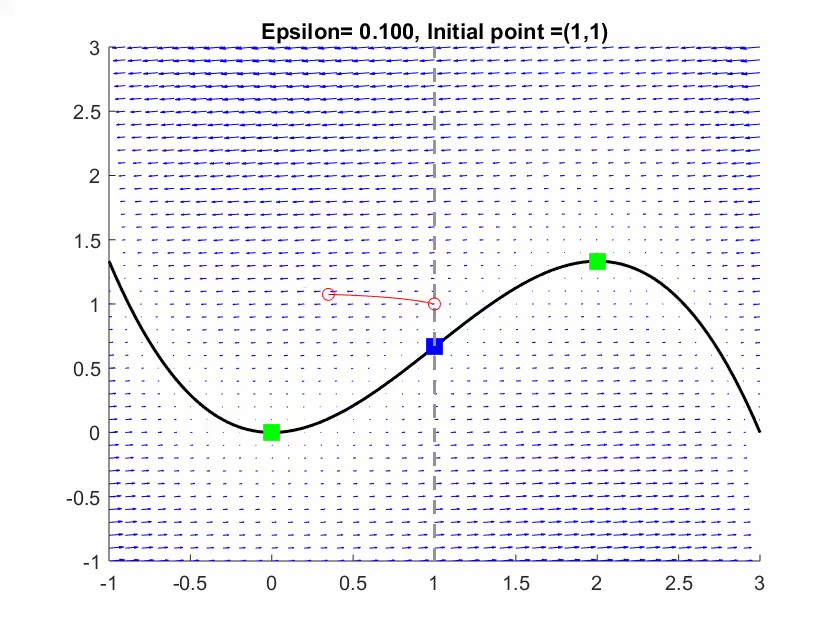
\includegraphics[width=.8\linewidth]{vdPhopf-Moment-1.jpg}
		\caption{The initial flow within the system.} \label{fig:timing1}
	\end{subfigure}
	\hfill
	\begin{subfigure}[t]{0.45\textwidth}
		\centering
		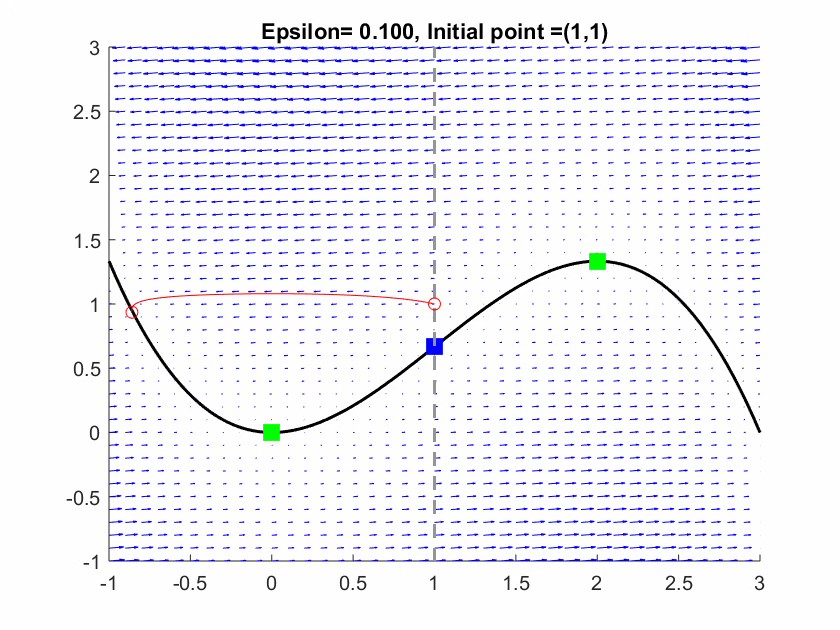
\includegraphics[width=.8\linewidth]{vdPhopf-Moment-2.jpg}
		\caption{The flow as it hits the slow manifold.} \label{fig:timing2}
	\end{subfigure}
	
	\vspace{1cm}
	\begin{subfigure}[t]{0.45\textwidth}
		\centering
		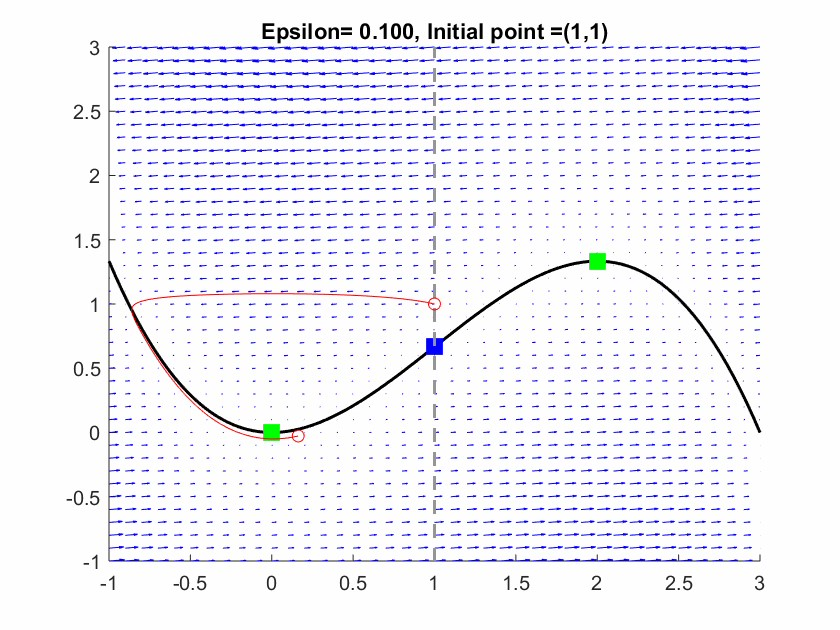
\includegraphics[width=.8\linewidth]{vdPhopf-Moment-3.jpg}
		\caption{The flow as it intersects with the fold point.} \label{fig:timing3}
	\end{subfigure}
	\hfill
	\begin{subfigure}[t]{0.45\textwidth}\centering
		% just an empty subfigure to shift C below A
		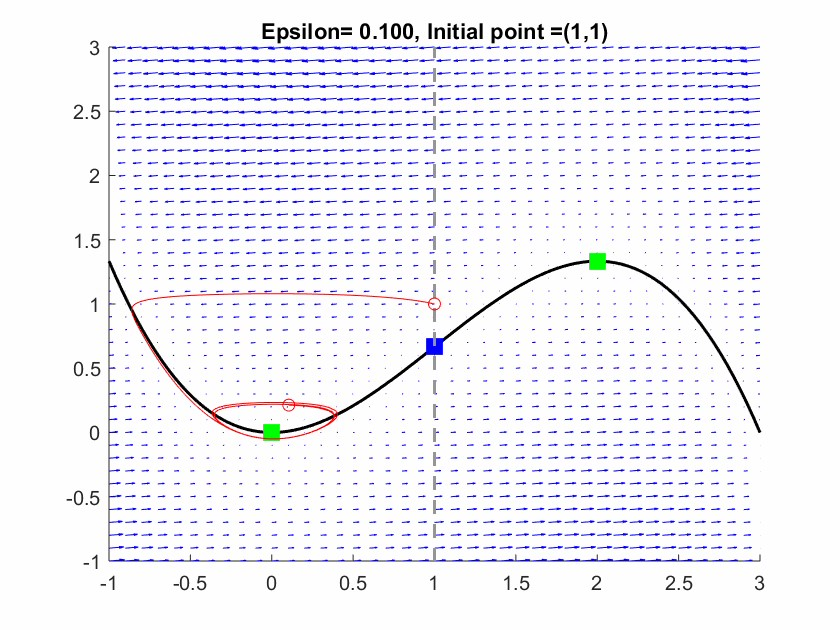
\includegraphics[width=.8\linewidth]{vdPhopf-Moment-4.jpg}
		\caption{The Hopf bifurcation due to the canard point.}\label{fig:timing4}
	\end{subfigure}\vspace{1cm}
	\begin{subfigure}[t]{0.45\textwidth}\centering
		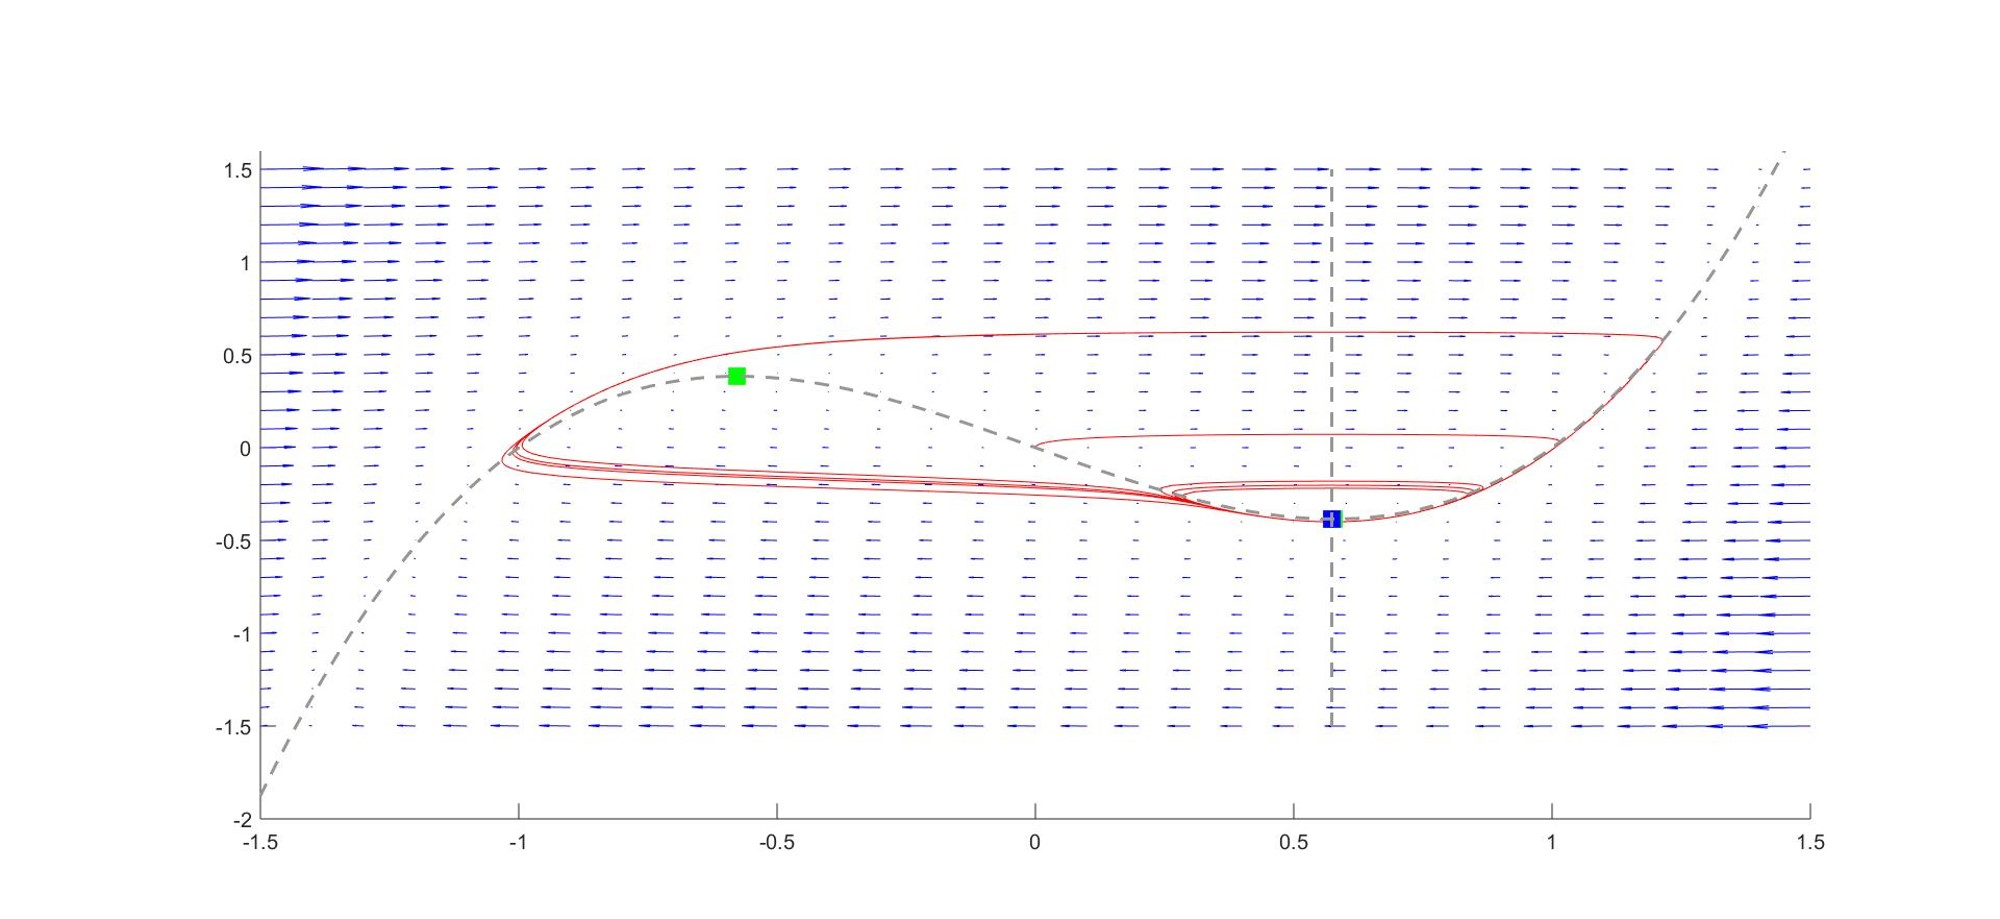
\includegraphics[width=.8\linewidth, height=6cm]{Code/behaviourswitch-pres}
		\caption{Growth of the Hopf bifrucation leading to the formation of a Canard explosion.}
		\label{fig: hopf growth}
	\end{subfigure}
	\caption{The trajectories associated with the canards case of the \vdp system.}
	\label{fig: 4 canard }
\end{figure}\newpage
From Figure \ref{fig: 4 canard } we can see the progression of our flow over the system. From Figure \ref{fig:timing1} we see that the flow starts at an initial condition of $ (x,y)=(1,1) $ and travels along the fast flow towards the attracting branch. Then from Figure \ref{fig:timing2} the flow has hit the attracting branch, where it then follows along the slow flow towards the fold point at $ (x,y)=(0,0) $, which is described by Figure \ref{fig:timing3}. Then from Figures \ref{fig:timing3} and \ref{fig:timing4} we can observe the Hopf bifurcation. This is because we make note that the canard point is present at $ -\lambda $, which in essence pushes the flow up the repelling branch (see Figure \ref{fig: Canard Point}) until the flow is sufficiently far from the fold point where it will then repel towards the attracting branch, starting the growing oscillations - Figure \ref{fig:timing4}. When the Hopf bifurcation is large we would then expect to see a jump in our solution to an attracting branch - Figure \ref{fig: hopf growth}.

%\begin{figure}[h!]\centering
%	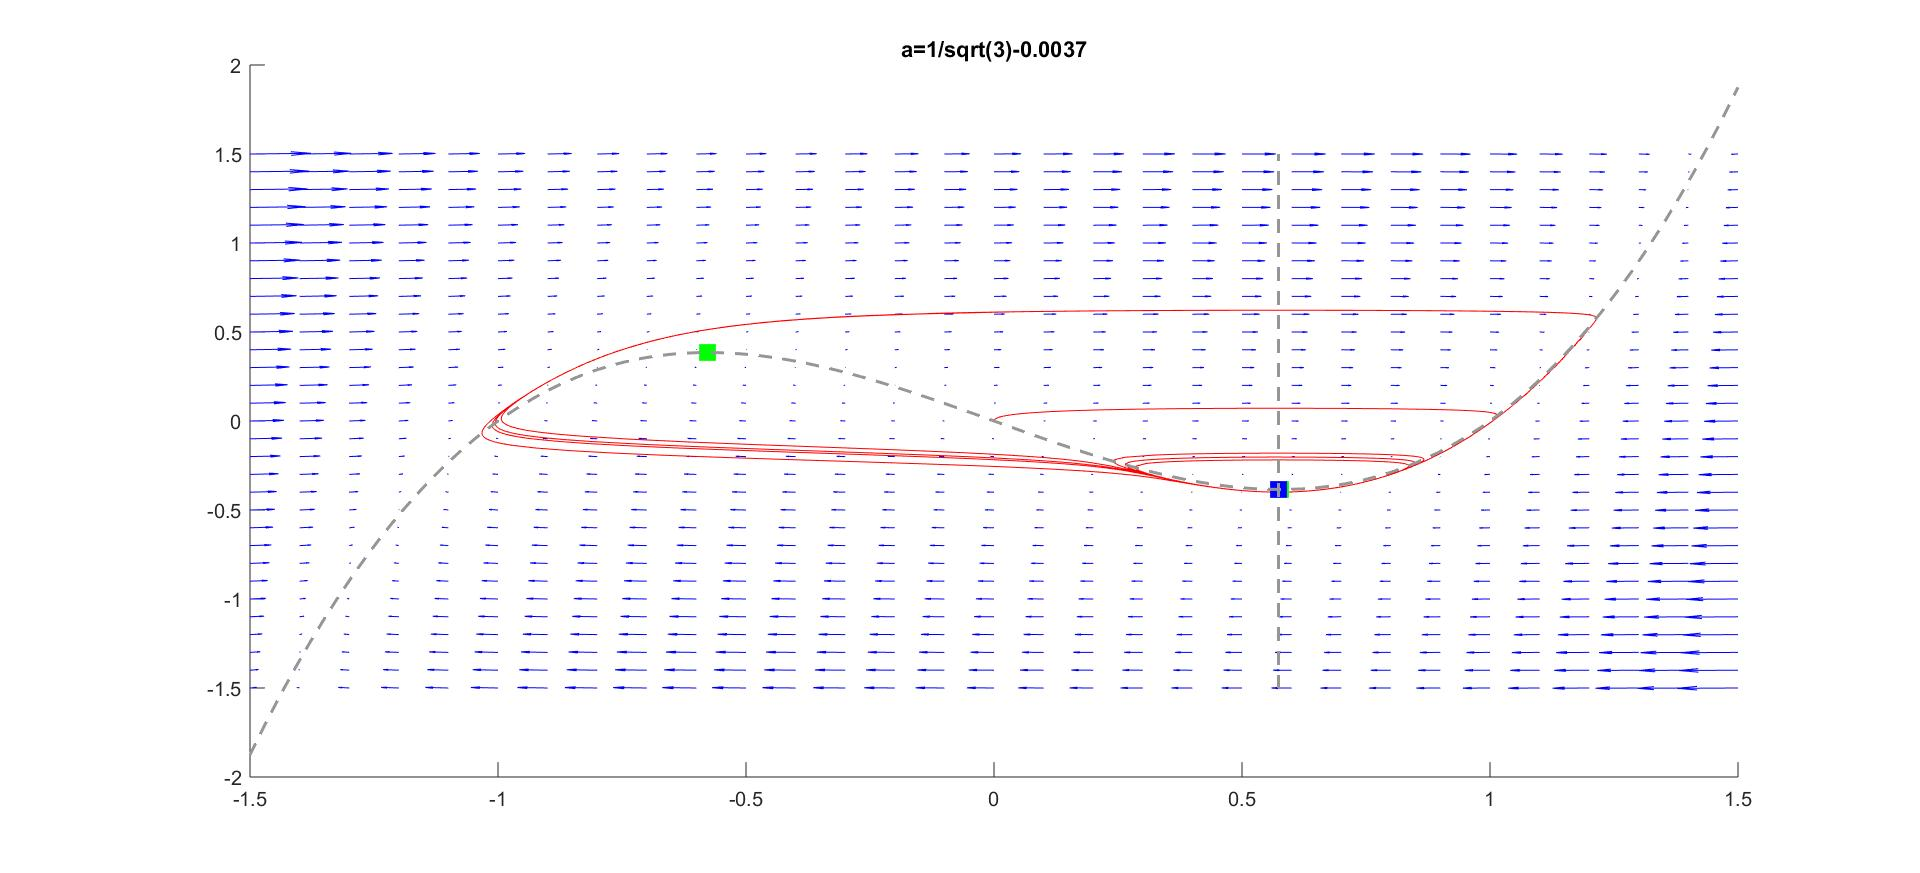
\includegraphics[height=8cm,width=6cm]{Code/behaviourswitch}
%	\caption{Growth of the Hopf bifrucation leading to the formation of a Canard explosion.}
%	\label{fig: hopf growth}
%\end{figure}\newpage
%
%Moreover, it is worth noting that our Hopf bifurcation only exists when we are in an arbitrarily small region, $ O(\epsilon) $, due to the local nature of the theorem \cite{Eckhaus}. 
%\begin{figure}[h!]\centering
%%	\includegraphics[]{}
%	\caption{Development of the Hopf Bifurcation. \textbf{Tom can you screenshot the flow in 4 places?}}
%	\label{fig: Hopf}
%\end{figure}
%Figure \ref{fig: 4 canard } shows that we have an unstable periodic solution within our canard system. In addition to this we know that our canard system will only exist within a small region of $ O(\epsilon) $ \citep{Eckhaus}. Moreover, we can see from Figure \ref{fig: Hopf} that our flow follows the expected path, as we saw in ++++++++++++++++++++++++\\
%%%%%%%%%%%%%%%%%%%%%%%%%%%%%%%%%%%%%%%%%%%%%%%%%%%%%%%%%%%%%%%%%%%%%%%%%%%%%%%%%%%%%%%%%%%%%%%%%%%%%%%%%%%%%%%%%%%%%%%%%%%%%%%%%%%%%%%%%%%%%%%%%%%%%%%%%%%%%%%%%%%%%%%%%%%%%%
%\subsubsection{Singular Hopf Bifurcation}\label{sec:singular-hopf-bifurcation}
%Furthermore, in the \vdp we are able to find a singular Hopf Bifurcation when $ \lambda=1 $. Then to model this behaviour we need to consider a small perturbation along the slow flow where we will have, from Equation \ref{eq: canard system},%discuss what the solutions for x is in the paper 
%\begin{equation}
%\dot{y}=\lambda-x+\bar{\nu} y,
%\end{equation}
%where $ \nu $ is of order $ O(\epsilon) $, thus small. We can immediately see that when $ \bar{\nu}=0 $ that we have our original flow at our equilibrium but we are now able to perturb our flow over a small domain, which are described in Figures \ref{fig: Hopf}. We can also see how our system behaves when our $ \nu $ is of larger order than $ O(\epsilon) $,
%
%\begin{figure}[h]\centering
%	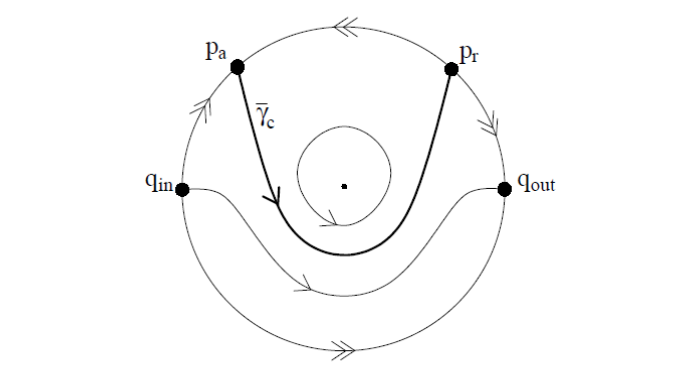
\includegraphics[height=6cm,width=10cm]{Images/CanardPointcircle}
%	\caption{The flow within our canard system \citep{krupa2001}.}
%	\label{fig: canard flow circle}
%\end{figure}\newpage
%where it is clear that our Hopf bifurcation is the periodic solution in the centre of Figure \ref{fig: canard flow circle} but we can see that below our special flow $ \bar{\gamma_c} $ (for the flow outside of the domain $ O(\epsilon) $),our solution traverses through our equilbrium into our fast flow as we would expect in our original system.

%%%%%%%%%%%%%%%%%%%%%%%%%%%%%%%%%%%%%%%%%%%%%%%%%%%%%%%%%%%%%%%%%%%%%%%%%%%%%%%%%%%%%%%%%%%%%%%%%%%%%%%%%%%%%%%%%%%%%%%%%%%%%%%%%%%%%%%%%%%%%%%%%%%%%%%%%%%%%%%%%%%%%%%%%%%%%%

%\subsubsection{Singular Hopf Bifurcation}\textbf{Does this section tie in anywhere else?}
%In this section we will further expand on our Hopf Bifurcation of the previous section (Section \ref{sec:effect-of-the-canard-point}). We note that we get a singular bifurcation iff our system is equivalent to Equation \ref{eq: Fast System}, \st $ \lambda=1 $. \citet{Eckhaus} discusses that our bifuraction will only exist within a small range of $ O(\epsilon) $. Then to model this behaviour we need to consider a small perturbation along the slow flow where we will have, from Equation \ref{eq: canard system},%discuss what the solutions for x is in the paper 
%\begin{equation}
%\dot{y}=\lambda-x+\bar{\nu} y,
%\end{equation}
%where $ \nu $ is of order $ O(\epsilon) $, thus small. We can immediately see that when $ \bar{\nu}=0 $ that we have our orignal flow at our equilbrium but we are now able to perturb our flow over a small domain, which are described in Figures \ref{fig: Hopf}. We can also see how our system behaves when our $ \nu $ is of larger order than $ O(\epsilon) $,
%
%\begin{figure}[h]\centering
%	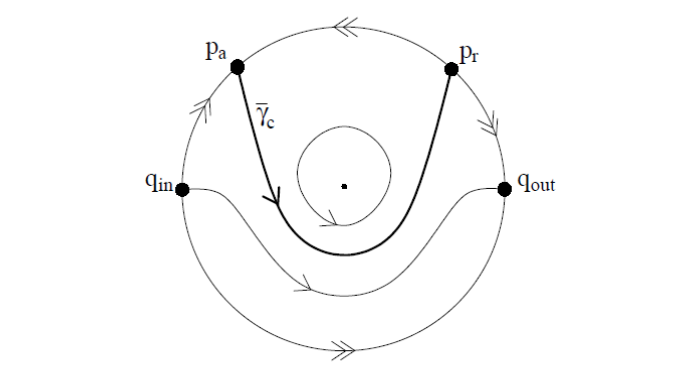
\includegraphics[height=6cm,width=10cm]{Images/CanardPointcircle}
%	\caption{The flow within our canard system \citep{krupa2001}.}
%	\label{fig: canard flow circle}
%\end{figure}\newpage
%where it is clear that our Hopf bifurcation is the periodic solution in the centre of Figure \ref{fig: canard flow circle} but we can see that below our special flow $ \bar{\gamma_c} $, our solution traverses through our equilbrium into our fast flow as we would expect in our original system.

%\newpage


\subsubsection{Separation of the Manifolds}\label{sec:separation-of-the-manifolds}
\begin{figure}[h!]\centering
	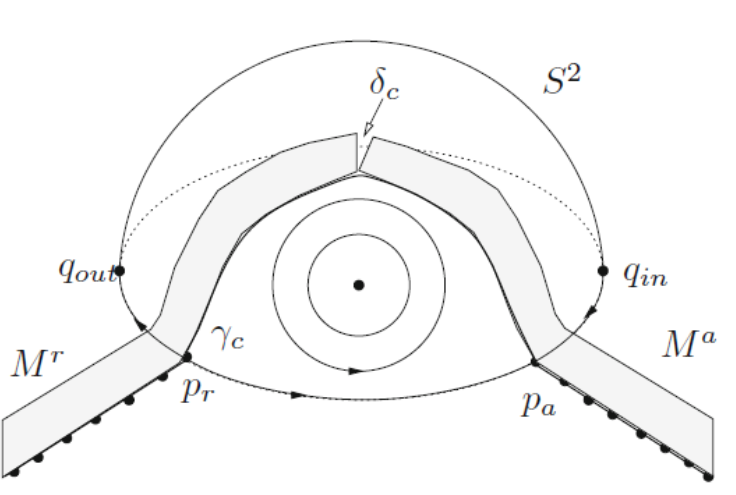
\includegraphics[height=8cm,width=10cm]{Images/Separation}
	\caption{Separation of $ M_a $ and $ M_r $ \citep{Kuehn}.}
	\label{fig: splitting}
\end{figure}%\newpage
%\textbf{Discuss splitting on the manifold}
Continuing on from the singular Hopf bifurcation we might find that the canard point forces our branches to split. In other words we are looking for when the attracting and repelling branches are no longer connected, as show in Figure \ref{fig: splitting}. To do this we would use Melnikov Computations to show that our manifolds split - see \textit{Extending Geometric Singular Perturbation Theory to Nonhyperbolic Points - Fold and Canard Points in Two Dimensions} \citep{krupa2001} for direct use. To discover whether we have a splitting between our branches we need to consider our $ y $ coordinates \wrt our second chart \st $ y_{a,2}(0)-y_{r,2}(0) $ is a distance function which can be written as $ D_c(r_2,\lambda_2)=H(0,y_{a,2}(0))-H(0,y_{r,2}(0)) $ as we note that $ \pd{}{y_2}H(0,y_2)\neq 0 $ \citep{krupa2001}. From here we can use the following proposition,
\begin{prop}
	[\citealp{krupa2001}]
	For a small enough $ \rho $ and $ \mu $ the distance function has the expansion
	\begin{equation*}
	D_c(r_2,\lambda_2)=d_{r_2}r_2+d_{\lambda_2}\lambda_2+O(2),
	\end{equation*}
	where we have defined,
	\begin{subequations}
		\begin{align}
		d_{r_2}&=\int_{-\infty}^{\infty}\text{grad}H(\gamma_{c,2}(t))^T\cdot G(\gamma_{c,2}(t))dt,\\
		d_{\lambda_2}&=\int_{-\infty}^{\infty}\text{grad}H(\gamma_{c,2}(t))^T\cdot (0,-1)^T,
		\end{align}
	\end{subequations}
	and our matrix $ G(\gamma_{c,2}(t)) $ in Section \ref{sec:dynamics-in-texorpdfstringk1k1} with $ \gamma_{c,2} $ as our critical trajectory. 
\end{prop}
Then, following the proof provided by \citet{krupa2001}, we find that we will have a split occurring between our branches if the canard falls outside of our domain of order $ O(e^{-\frac{c}{\epsilon}}) $ \st $ D_c(r_2,\lambda_2)\neq 0 $. We can calculate these explicitly for the the \vdp system by using Equations \ref{eq: const of motion}, \ref{eq: gamma c2} and $ G(x_2,y_2)=(-\frac{x_2^3}{3},0)^T $ \st we have,

	\begin{align*}
		d_{r_2}&=\int_{-\infty}^{\infty} \nabla\left(\frac{1}{2}e^{-2y_2}\left(y_2-x^2_2+\frac{1}{2}\right)\right)^T\cdot\left((-\frac{x_2^3}{3},0)^T\right)\bigg|_{\gamma_{c,2}} \text{dt}\notag\\
%	&=\int_{-\infty}^{\infty}\left(-\frac{\exp\left(-\frac{t^2}{2}+1\right)}{2}.\frac{\exp\left(-\frac{t^2}{2}+1\right)}{2}\left(\frac{t^2}{4}-\frac{1}{2}-\frac{t}{2}\right)\right)
		&=-\frac{e}{16}\int_{-\infty}^{\infty}t^4e^{-\frac{T^2}{2}}dt,
	\end{align*}

noting $ \nabla(H)= $
Now the task is to show that $ d_{r_2} $ is finite, we do this by using integration by parts to find,
\begin{equation}
d_{r_2}=	\frac{e}{16}\int_{-\infty}^{\infty}e^{-\frac{T^2}{2}}dt=\frac{e\sqrt{2\pi}}{16}<\infty,
\end{equation}
where we note that we have made use of the Guassian Integral \citep{GausIntegral} to show finiteness. We then apply an analogous approach to $d_{\lambda_2} $ \st, 
\begin{align}
		d_{\lambda_2}&=\int_{-\infty}^{\infty} \nabla\left(\frac{1}{2}e^{-2y_2}\left(y_2-x^2_2+\frac{1}{2}\right)\right)^T\cdot\left((0,-1)^T\right)\bigg|_{\gamma_{c,2}} \text{dt}\notag\\
		&=-\frac{e}{2}\int_{-\infty}^{\infty} e^{-t^2}dt=-\frac{e\sqrt{2\pi}}{2}<0,
\end{align}
where we have used the same techniques as above where we note that $ d_{\lambda_2} $ is also finite. Combining the above yields that our distance function is,
\begin{equation}
	D_c(r_2,\lambda_2)=\frac{e\sqrt{2\pi}}{16}r_2-\frac{e\sqrt{2\pi}}{2}\lambda_2+O(2),
\end{equation}  
whereby we have that the manifolds in the \vdp system split for $ \lambda_2\neq\frac{r_2}{8} $ otherwise our branches are connected, as shown in the prior simulations. If the manifold splits then we would find that the manifold is similar to Figure \ref{fig: splitting} whereby the flow will either jump off fracture - see Figure \ref{fig: vdp flow diagram e} - or the flow will be trapped in the canard region and then be repelled back to the attracting manifold, as we see with our connected system - Figure \ref{fig: 4 canard }. 





